%************************************************
\chapter{Flash simulation of samples with Normalizing Flows}\label{ch:fs} % $\mathbb{ZNR}$
%************************************************

Having discussed the importance and the challenges of event simulation at LHC, and having described the Deep Learning Normalizing Flows approach, we dedicate this chapter to the practical implementation of an end-to-end sample generator.

The code discussed in the following sections and used in this work may be found online \href{tbd}{here}\footnote{tbd}.

\section{Target variables}

As we discussed in Section \ref{sec:targets}, we choose to target the VBF Channel of H$\rightarrow\mu^+\mu^-$. Thanks to the clear signature, we only needed to simulate jets and muons out of all the possible objects in a NanoAOD. The present section serves as a discussion of the chosen variables to be simulated with our approach.

However, because our Machine Learning Models need a large amount of training data, having already been simulated through FullSim in large numbers, the VBF signal MC data samples were not sufficient for our task. We thus turned to the t$\overline{\text{t}}$ process.

\subsection{The t$\overline{\text{t}}$ process}
The top quark is an important component of the standard model, especially because of
its large mass, and its properties are critical for the overall understanding of the theory. Measurements of the top quark-antiquark pair (t$\overline{\text{t}}$) production cross section test the predictions of
quantum chromodynamics (QCD), constrain QCD parameters, and are sensitive to physics beyond the SM. With a cross-section of $\approx 900$ pb at 13 TeV , the t$\overline{\text{t}}$ process is also \emph{the dominant SM background to many searches for new
physical phenomena}, and its precise measurement is essential for claiming new discoveries.
The copious top quark data samples produced at the CERN LHC enable measurements of the t$\overline{\text{t}}$
production rate in extended parts of the phase space, and differentially as a function of the kinematic properties of the t$\overline{\text{t}}$ system. Inclusive and differential cross section measurements from
proton-proton (pp) collisions at centre-of-mass energies of 13 TeV have been reported by
the CMS collaboration in \cite{Sirunyan_2017}.

\graffito{were our samples dijets or mixed?}
Top quarks decay almost exclusively into a W boson and a b quark. The W may then decay in either a q$\overline{\text{q}}$ or a lepton and its corresponding neutrino, ensuring that the events will be well populated with both jets and muons, our simulation targets. \graffito{do we want a figure for ttbar?}

%\begin{figure}
    %\centering
    %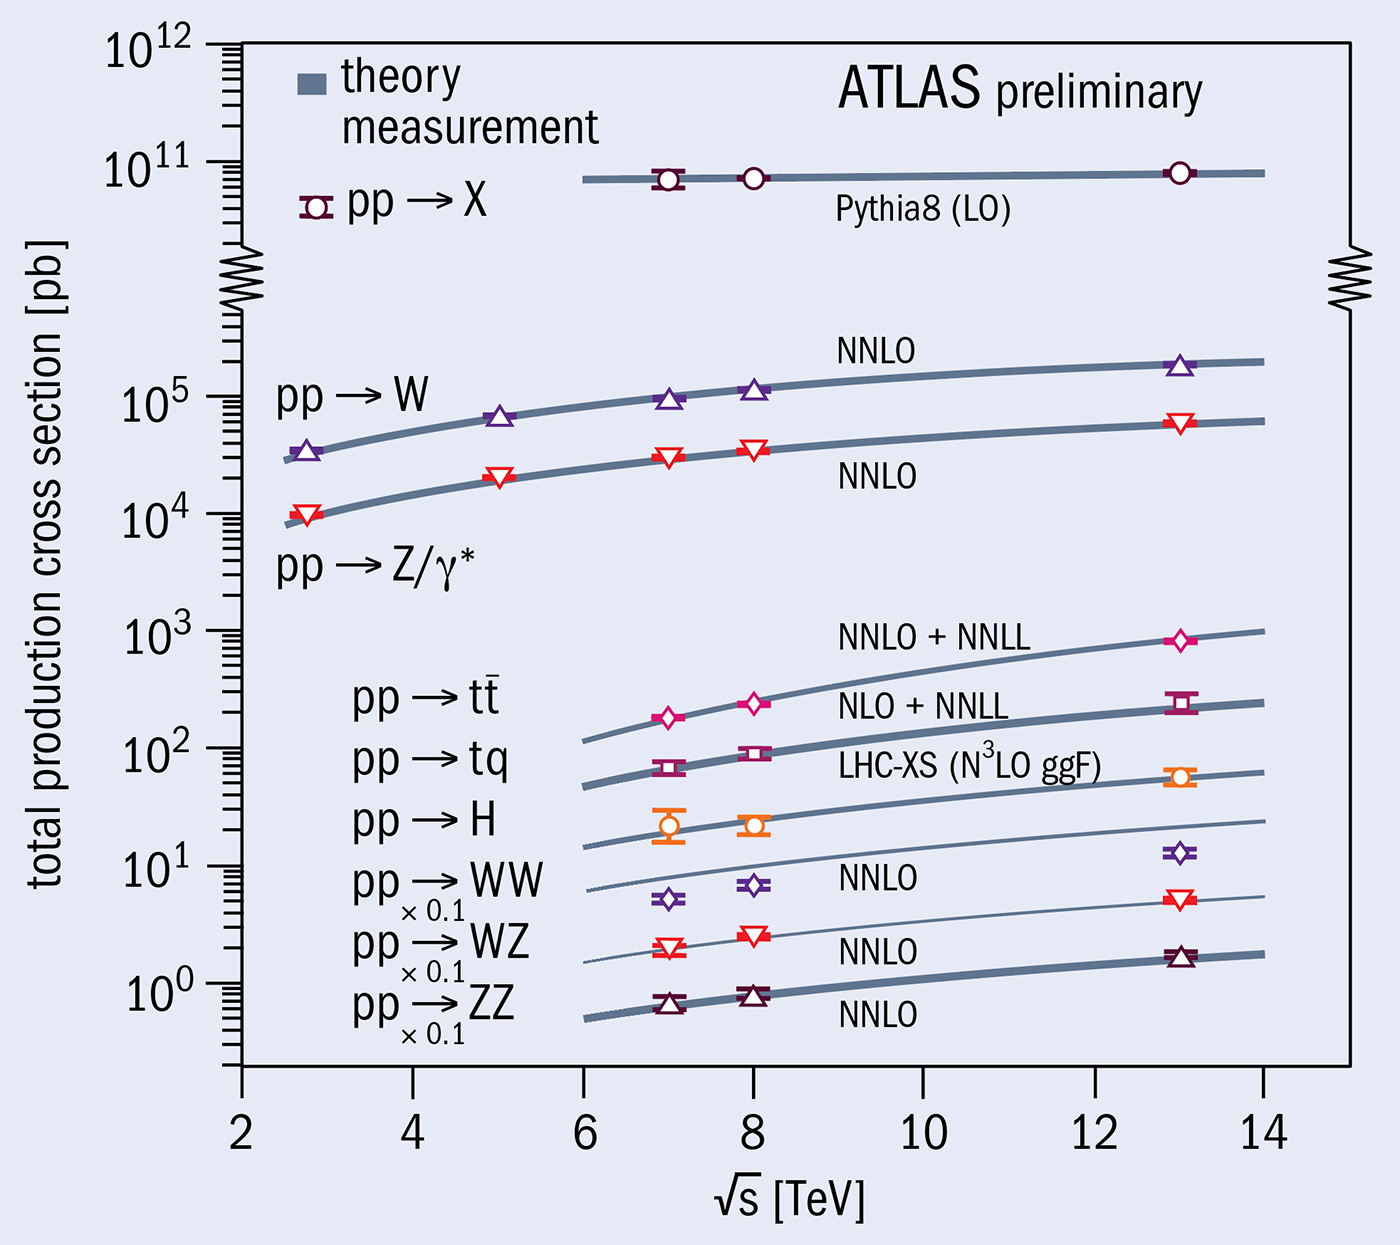
\includegraphics[scale=0.2]{gfx/ch5/CCMarApr_LHC10_fig2.jpg}\quad
    %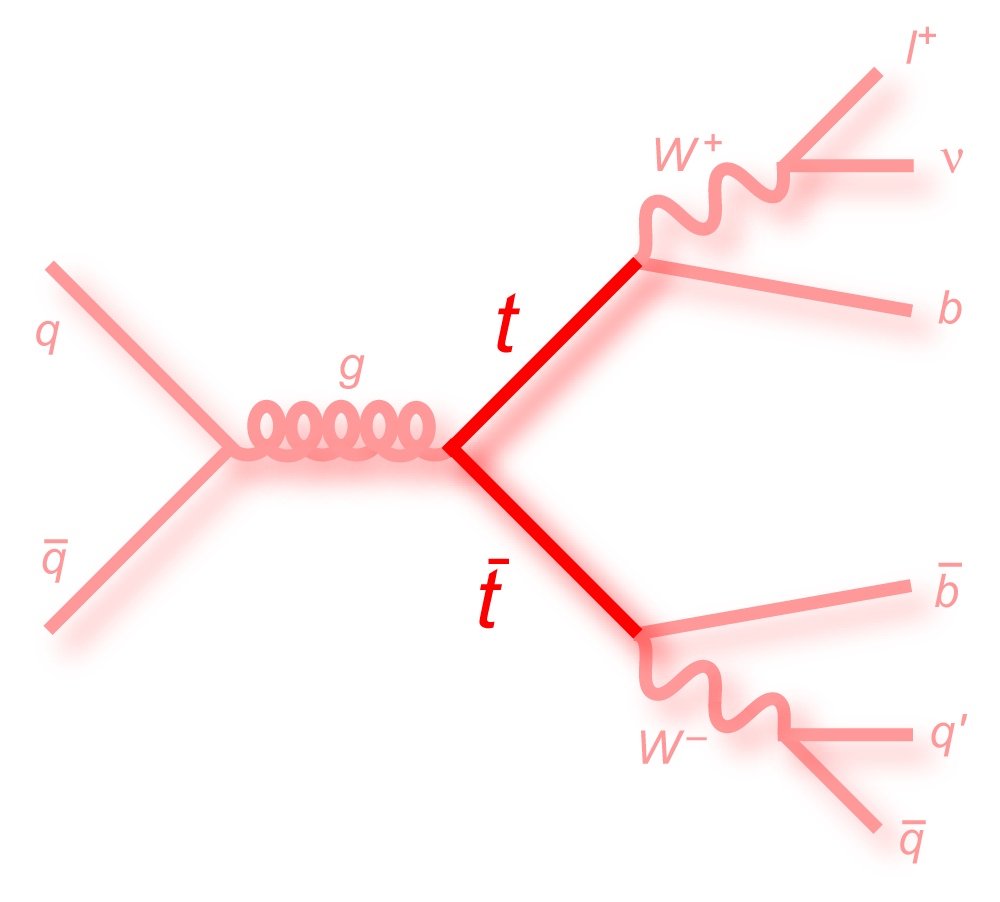
\includegraphics[scale=0.3]{gfx/ch5/feynman_ttbar_ljets_longt.png}
    %\caption[t$\overline{\text{t}}$ diagram]{ The t$\overline{\text{t}}$ process is dominating the cross sections at LHC, making it one of the leading SM background processes. Bottom: the production diagram for proce}
    %\label{fig:ttfig}
%\end{figure}

Having at our disposal a large set of FullSim MC NanoAOD samples for t$\overline{\text{t}}$ dijet/at least one jet(??) events, we used these to \emph{train} our models on the two target objects.

\subsection{Jets}

As discussed in Section \ref{sec:nanoaod}, a NanoAOD contains both the Jet objects, i.e. final-state reconstructed jets, and the GenJet objects, the jets resulting from a generator and which will pass through all the steps of the FullSim simulation chain, which are either matched to Jet objects, or may end-up unmatched because of limitations in the matching algorithms and the previous simulation steps. For the moment, we disregard the problem of \emph{fake jets}, that is Jet objects which are not reconstructed from a GenJet object but are instead due to noise or errors in clustering algorithms.

The idea is being able to directly generate correctly distributed Jet objects starting from noise, for stochasticity,  but also from the values of a corresponding GenJet, as a physical-informed input for the network (a process known as \emph{conditioning}): knowing just the diagram-level physics of some process, we are going to skip the Simulation, Digitization and Reconstruction steps.


With the use of \texttt{C/C++} code (name of script) for the \texttt{ROOT} data analysis framework \cite{Brun:491486}, we processed the NanoAOD files and extracted all the Jet objects matched to a GenJet object, across all the events in the file. Because of the large number of variables, we selected a meaningful subset, containing all the necessary information for our test analysis.

First of all, we selected the following 14 GenJet variables for conditioning the generation: 
\graffito{do we want plots of vars?}

\begin{outline}
\1 \emph{The physical properties} of the GenJet, that is \texttt{Eta}, \texttt{Phi}, \texttt{Mass}, \texttt{Pt}, the \texttt{PartonFlavour}, giving the parton content of a GenJet as a specific number and the \texttt{HadronFlavour}, describing the hadron content in a similar way;
\1 \emph{Engineered, physical-informed variables} which we designed to express interesting physical properties of the GenJet. Computing the $\Delta$R separation between the GenJet and the GenMuons present in the event, we selected the first and second \emph{closest muons}, and we computed the following quantities for each one:
\2 \texttt{Dr}, giving the separation from the GenJet, \texttt{DEta}, the $\eta$ difference from the GenJet, \texttt{DPt}, the $p_T$ difference from the GenJet, \texttt{DPhi}, the $\phi$ difference from the GenJet, which is to be computed accounting for the \emph{periodicity} of the $\phi$ variable;

\1 If no GenMuons were present within a cone of $\Delta$R = 0.5 from the GenJet, the corresponding values were set to a user-defined maximum.

\end{outline}

Then, we selected the following 17 target variables for the matched reconstructed Jet objects:

\begin{outline}
\1 \emph{The physical properties} of the Jet \emph{with regard to} the ones of the matched GenJet: \texttt{EtaMinusGen}, the $\eta$ difference , \texttt{PhiMinusGen}, the $\phi$ difference, \texttt{MassRatio}, the ratio of the jet and GenJet masses, \texttt{PtRatio}, the ratio of $p_T$s. This was done because the Simulation and Reconstruction steps are expected to introduce corrections w.r.t. the GenJet distributions, easier to learn when considering these quantities. As an additional variable, the Jet \texttt{Area}, a measure of its susceptibility to radiation, like pileup or underlying event, was added as well;

\graffito{what does btag -1 stand for?}
\1 The most relevant \emph{b-tagging and c-tagging algorithms scores}: \texttt{btagCMVA}, \texttt{btagCSVV2}, \texttt{btagDeepB}, \texttt{btagDeepC}, \texttt{btagDeepFlavB} and \\\texttt{btagDeepFlavC}, which indicate with a score ranging from 0 to 1 whether the Jet contains the respective quark or not, a very significant information for performing event selection during an analysis. Some values may be offsetted to -1 to indicate ???;

\1 The \texttt{bRegCorr}, the $p_T$ correction for b-jet energy regression;

\1 The \texttt{qgl} score for the Quark vs Gluon likelihood discriminator;

\1 The \texttt{jetID} and \texttt{puID} ID flags indicating relevant characteristics of the jet and the Pile-Up.
\end{outline}
\subsection{Muons}

For muons we performed the same procedure, taking only those muons matching to GenMuon objects (a GenParticle object with pdgId value of $\pm$13). 

We selected 30 GenMuon variables for conditioning:

\begin{outline}
\1 \emph{The physical properties} of the GenMuon, that is \texttt{Eta}, \texttt{Phi}, \texttt{Charge} and \texttt{Pt};

\1 \emph{The 14 GenParticle status flags}, a series of \texttt{statusFlags} stored bitwise, with each bit having a different physical interpretation such as \emph{isTauDecayProduct}, \emph{fromHardProcess}, etc. or some information regarding the position of the object in the detector (e.g. \emph{isLastCopy}, indicating that this is the last copy of the GenPart in the detector to be used for the analysis);

\1 \emph{Engineered, physical-informed variables} which we designed to express interesting physical properties of the GenMuon. Computing the $\Delta$R separation between the GenMuon and the GenJets present in the event, we selected the first \emph{closest GenJet}, and we computed the following quantities:
\2 \texttt{Dr}, giving the separation from the GenJet, \texttt{DEta}, the $\eta$ difference from the GenJet, \texttt{Pt}, the $p_T$ of the GenJet,
\texttt{DPhi}, the $\phi$ difference from the GenJet, which is to be computed accounting for the \emph{periodicity} of the $\phi$ variable and finally the \texttt{Mass} of the closest GenJet;

\1 A series of 6 \emph{ Event level variables regarding Pile-Up}:\\ \texttt{Pileup\_gpudensity}, the Generator-level PU vertices/mm,\\ \texttt{Pileup\_nPU}, the number of pileup interactions that have been added to the event in the current bunch crossing, \texttt{Pileup\_nTrueInt}, the true mean number of the poisson distribution for this event from which the number of interactions each bunch crossing has been sampled, \texttt{Pileup\_pudensity}, PU vertices/mm, \texttt{Pileup\_sumEOOT}, the number of early out of time pileup and \texttt{Pileup\_sumLOOT}, the number of late out of time pileup;
\end{outline}

Then we selected 22 target variables for the Muon objects:

\begin{outline}
\1 \emph{The physical properties} of the muon \emph{with regard to} the ones of the matched GenMuon: \texttt{EtaMinusGen}, the $\eta$ difference , \texttt{PhiMinusGen}, the $\phi$ difference, \texttt{PtRatio}, the ratio of $p_T$s. This was done because the Simulation and Reconstruction steps are expected to introduce corrections w.r.t. the GenMuon distributions, easier to learn when considering these quantities. As an additional variable, the \texttt{ptErr}, the $p_T$ error for the muon track, was selected as well;

\1 Six \emph{impact parameters} with regard to the primary vertex: \texttt{dxy}, \texttt{dxyErr}, \texttt{dz}, \texttt{dzErr}, the 3D impact parameter \texttt{ip3d} and its significance \texttt{sip3d}, all expressed in cm;

\1 Some \emph{Boolean flags}: \texttt{isGlobal}, \texttt{isPFcand}, identifying the muon as a Particle Flow candidate, \texttt{isTracker};

\1 A series of \emph{isolation variables} returned by the Particle Flow algorithm: \texttt{pfRelIso03\_all}, \texttt{pfRelIso03\_chg} and \texttt{pfRelIso04\_all};

\1 The \emph{variables related to the closest jet}: \texttt{jetPtRelv2}, indicating the relative momentum of the lepton with respect to the closest jet after subtracting the lepton and \texttt{jetRelIso}, the relative isolation in matched jet;

\1 A series of \emph{ID scores}: \texttt{mediumID}, \texttt{softMVA} score and its cut-based ID \texttt{softMVAId}, \texttt{softId};
\end{outline}

\subsection{Extraction and preprocessing}

With the use of \texttt{C/C++} code (name of script) for the \texttt{ROOT} data analysis framework \cite{Brun:491486}, we processed the NanoAOD files and extracted all the Jet objects matched to a GenJet object and the Muon objects matched to a GenMuon across all the events in the file. This operation can be performed rather quickly thanks to the \emph{compiled} language being used and the powerful \texttt{ROOT::RDataFrame()} class, offering a modern, high-level interface for the manipulation of data stored in a NanoAOD \texttt{TTree}, as well as \emph{multi-threading} and other low-level optimisations.
The output of the \emph{extraction} step is another \texttt{.root} file containing just the selected objects.

The resulting file is still organized according to the Events structure. Besides, we know that many machine learning algorithms work best when specific distributions are \emph{preprocessed} according to specifc criteria. Normalizing Flows are no exception. Specifically, there are four key features which should be accounted for and modified through preprocessing before training:

\begin{figure}
    \centering
    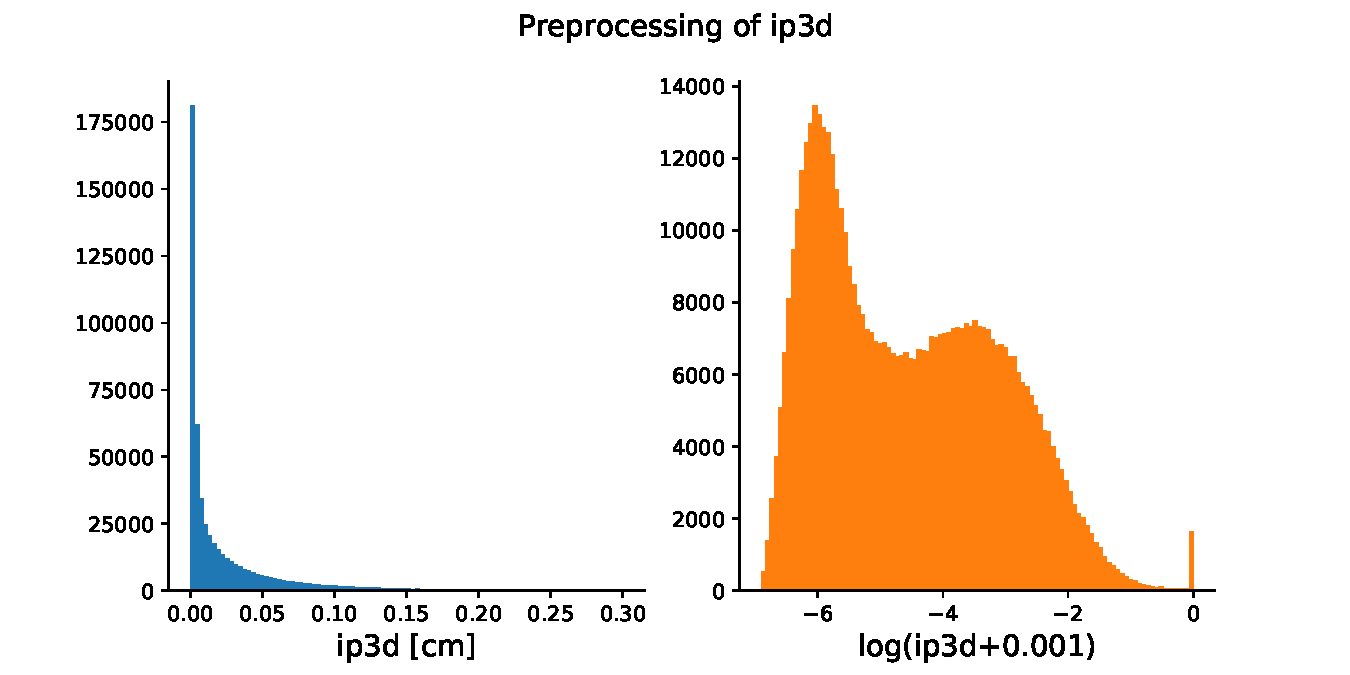
\includegraphics[width=\columnwidth]{gfx/ch5/preproce.pdf}
    \caption[Preprocessing]{Sharply peaked distribution are being converted to more broad ones during the preprocessing step. In this example the \texttt{ip3d} variable gets transformed as log(\texttt{ip3d}+0.001).}
    \label{fig:preproce}
\end{figure}

\begin{outline}
\1 Because NF are learning actual pdfs, \emph{large gaps} between values of the distribution may disturb training and trick the network to \emph{bridge} the extremes of the distribution by creating spurious samples in the gap. When possible, the gaps should be reduced and the values packed closer together;

\1 As NF work with pdfs, they are not well suited to deal with \emph{discrete} distributions. Thus, we should apply a process known as \emph{dequantization}, that is applying some sort of smearing to the discrete values to make them similar to those sampled from a continuous distribution;

\1 For similar resons as before, when possible it would be beneficial to widen and normalize sharply peaked distributions through invertible transforms such as log(x). If well separated, eventual peaks may be dequantized as well;

\1 Finally, we opted for \emph{saturating} long tails of distributions to some limiting values, in order to make it easier for the model to learn the pdf in the more populated region.
\end{outline}

Apart from possibly dequantization, we stress that all of this transformations were implemented to make training easier but are not strictly necessary--the models revealed themselves as powerful enough to deal with complex, sharply peaked, long tailed distributions. However, having already implemented the preprocessing pipeline and because it did not introduce a big overhead in the procedure, we decided to keep it for the present work. An example of one of the possible preprocessing operations is shown in Figure \ref{fig:preproce}.

All of these transforms may be implemented with a clear and natural syntax in the \texttt{Python} programming language, specifically thanks to the \texttt{pandas} package \cite{reback2020pandas}, which implements a convenient dataframe structure. We thus open the \texttt{.root} file directly in a \texttt{Python} script through the \texttt{uproot} package \cite{jim_pivarski_2022_6791281}, discard the Events structure to obtain a simple table with one object per line, perform the preprocessing as discussed above and save the output in \texttt{.hdf5} format for the training.

\section{Models design}
This section describes the implementation  details for the two architectures--the one responsible for the generation of jets and the one targeting muons. We discuss the software choices and then the model specifics and trainings.

\subsection{Software and packages}

We initially planned to use another class of generative models, that is Generative Adversarial Networks. However, after discovering the work of Dr. Stephen Green \cite{stephen_green_2021_4558988} we realized that Normalizing Flows were better suited to our task, as they suffered from less training instabilities and allowed us to directly learn the underlying distributions with an easily interpretable loss function.

The models are implemented following Dr. Green's example: the \texttt{Python} package \texttt{nflows} \cite{conor_durkan_2020_4296287} defines the Classes for Rational Quadratic Spline Normalizing Flows, integrating them for use with the popular ML research package \texttt{Pytorch} \cite{NEURIPS2019_9015}. We obviously had to perform several attempts to optimize the hyperparameters choices for our use case, a long and complicated process which resulted in the architectures presented below.

\subsection{Architectures and trainings}

\begin{figure}
    \centering
    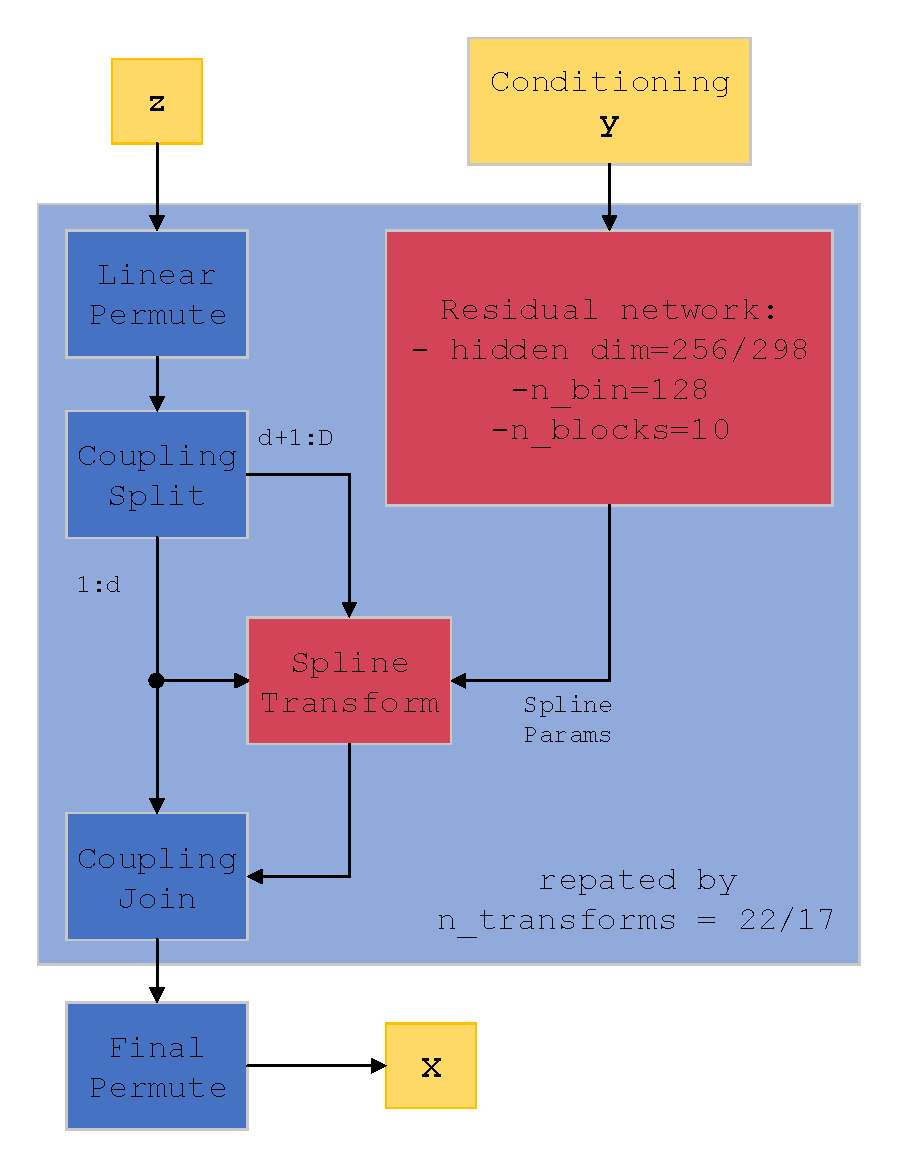
\includegraphics[width=\columnwidth]{gfx/ch5/nfmodel.pdf}
    \caption[Actual NF model]{The NF models are quite large and complex. A number of transforms equal to that of the target variables is performed. The normally distributed inputs \textbf{z} are permuted for each step and then splitted in half, sending half as parameters and half as argument of the \emph{spline transform}. The conditioning variables \textbf{y} are sent as input to a complex 10 layer network (different for each transform) which defines the parameters for the spline. Everithing is repeated until the last step where we permute back to the original order and output the targets \textbf{x}. Where two numbers are separetad by a slash, the first refers to the muons model, the second to the jets one.}
    \label{fig:nfmodel}
\end{figure}

Figure \ref{fig:nfmodel} shows the final models employed in this work. 
As discussed in Section \ref{sec:couplay}, in order to reduce the computational complexity of the Jacobian, we implemented the total transformation as a chain of single, subsequent splines transformations, each acting on just half of the input, while the latter half is kept unchanged and serves as additional parameters for the splines. This has the additional advantage of ensuring good \emph{correlations} between the various variables, as the transformation for one of them will end up depending on every other variable as long as we implement a number of transformation equal to the number of variables and we permute the order linearly before each spline.

For each spline, the normally distributed inputs \textbf{z} are permuted and then splitted in half, sending half as parameters and half as argument of the \emph{spline transform}. The conditioning Gen-level variables \textbf{y} are sent as input to a complex 10 layer fully-connected network (a different one for each transform) which defines the parameters for the spline. Its most relevant hyperparameters are the \emph{hidden\_dim}, the number of nodes per hidden layer, set to 256 for the muons model and to 298 for the jets one, the \emph{n\_bin}, the number of bins for the spline, set to 128 for both models and the \emph{n\_blocks} set to 10 for both and defining the number of hidden layers.
Each network was defined with \texttt{ReLU} activation function and setting \texttt{batch\_norm=True}.
\graffito{need to discuss batchnorm AND cosine\_annealing in ch3}

We would like to emphasize the fact that because \emph{each transform} defines a separate network for learning the optimal spline parameters, the final models are quite large, especially for physics-based application standards. The muons model exceeds 54e6 trainable parameters (54,988,164 parameters, corresponding to the various weights of the neurons in each layer), while the jets model totals in at 47,986,595 parameters. These large models were trained on around 5e6 muons or jets objects extracted as explained above, and the \emph{losses} were monitored at each epoch on a separate \emph{validation set} of about 4e5 samples to ensure that the models were not being over-optimized for the training set.

As our \emph{optimizer} algorithm we choose the de-facto standard in the field, the \texttt{Adam} algorithm \cite{https://doi.org/10.48550/arxiv.1412.6980}, a complex and powerful algorithm for models optimization still based on the same basic principles of Section \ref{sec:backprop}, with an initial \emph{learning rate} of xxx, reduced during training by the \emph{cosine annealing} procedure.


\begin{figure}
    \myfloatalign
    \subfloat[]
    {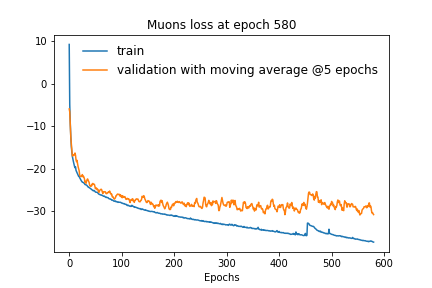
\includegraphics[width=.45\linewidth]{gfx/ch5/lossesmuons.png}} \quad
    \subfloat[]
    { 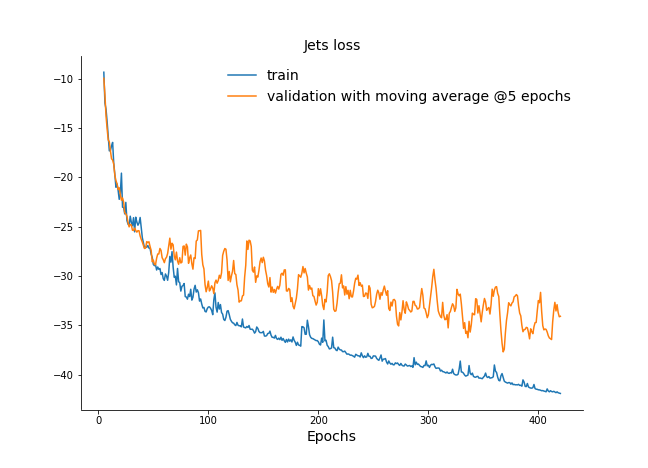
\includegraphics[width=.45\linewidth]{gfx/ch5/lossesjets.png}} \\
    \caption[Models losses]{stuff.}\label{fig:losses}
    
\end{figure}

\section{Results}

\subsection{1d distributions and correlations}

\subsection{Conditioning}

\section{A prototype end-to-end analysis sample generator}
